

\documentclass{article}

\usepackage{multicol}
\setlength{\columnsep}{1.2cm}
\usepackage{pgfplots}
\pgfplotsset{compat = newest}
\usepackage{titlesec}
\usepackage{graphicx}
\usepackage{wrapfig}
\usepackage{amsfonts}
\usepackage{tikz}
\usepackage{amssymb}
\usepackage{amsfonts}
\usepackage{amsmath}


\title{Intro to Functions}
\author{Anna Denisova}
\date{2023}

\begin{document}

\maketitle
\tableofcontents

%----------------------------------------------------------

\newpage
\section{Function Definitions}

\textbf{Relation} - Any relationship (set of ordered pairs) \\
\textbf{Function} - A relation that maps each input (x) to exactly one output (y)\\
\textbf{Finite} - Countable (discrete)\\
\textbf{Infinite} - Uncountable \\
\textbf{Mapping Diagram} - A visual representation of inputs and outputs (finite only)\\
\textbf{Vertical Line Test (VLT)} - A relation is not a function if you can draw a vertical line and cross the graph more than once. ($\because$ VLT fails/passes $\therefore$ this is/is not a function.)\\
%----------------------------------------------------------

\newpage
\section{Function Notation}

\textbf{$f(x)$}
\begin{itemize}
    \item used in place of y in equations
    \item helpful for identifying equations and input used
\end{itemize}


%----------------------------------------------------------

\newpage
\section{Parent Functions}

    \begin{multicols}{2}
    \noindent
    \textbf{Quadratic Function}\\
    $y = x^{2}$\\
    Key Points = \{(-2,4), (-1,1), (0,0), (1,1), (2,4)\}\\
    Domain = \{$\mathbb{R}$\} \\
    Range = \{$y \epsilon  \mathbb{R} | y \geq 0$\} \\\\

    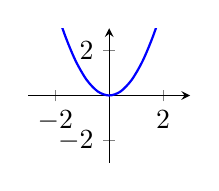
\begin{tikzpicture}
        \begin{axis}[scale = 0.3, axis lines = center, xmin=-3, xmax=3, ymin=-3, ymax=3]
            \addplot[blue,smooth, thick] {x^2};
        \end{axis}
    \end{tikzpicture}\\

    \noindent
    \textbf{Root Function}\\
    $y = \sqrt{x}$\\
    Key Points = \{(0,0), (1,1), (4,2), (9,3)\}\\
    Domain = \{$x\epsilon \mathbb{R} | x \geq 0$\} \\
    Range = \{$y \epsilon  \mathbb{R} | y \geq 0$\} \\
    
    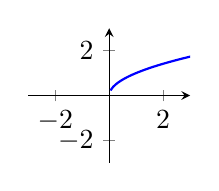
\begin{tikzpicture}
        \begin{axis}[ axis lines = center, xmin=-3, xmax=3, ymin=-3, ymax=3, scale = 0.3, samples=100]
            \addplot[blue, smooth, thick, unbounded coords = jump] {sqrt(x)};
        \end{axis}
    \end{tikzpicture}\\

    \noindent
    \textbf{Cubic Function}\\
    $y = x^{3}$\\
    Key Points = \{(-2,-8), (-1,-1), (0,0), (1,1), (2,8)\}\\
    Domain = \{$\mathbb{R}$\} \\
    Range = \{$\mathbb{R}$\} \\

    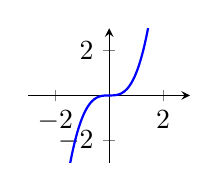
\begin{tikzpicture}
        \begin{axis}[ axis lines = center, xmin=-3, xmax=3, ymin=-3, ymax=3, scale = 0.3, samples=100]
            \addplot[blue, smooth, thick, unbounded coords = jump] {x^3};
        \end{axis}
    \end{tikzpicture}\\

    \noindent
    \textbf{Absolute Value Function}\\
    $y = |x|$\\
    Key Points = \{(-2,2), (-1,1), (0,0), (1,1), (2,2)\}\\
    Domain = \{$\mathbb{R}$\} \\
    Range = \{$y \epsilon  \mathbb{R} | y \geq 0$\} \\

    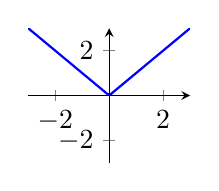
\begin{tikzpicture}
        \begin{axis}[ axis lines = center, xmin=-3, xmax=3, ymin=-3, ymax=3, scale = 0.3, samples=100]
            \addplot[blue, smooth, thick, unbounded coords = jump] {abs(x)};
        \end{axis}
    \end{tikzpicture}\\

    \noindent
    \textbf{Reciprocal Function}\\
    $y = \frac{1}{x}$\\
    Key Points = \{(-2,-$\frac{1}{2}$), (-1,-1), (-$\frac{1}{2}$,-2), ($\frac{1}{2}$,2), (1,1), (2,$\frac{1}{2}$)\}\\
    Domain = \{ $x \epsilon \mathbb{R} | x \neq 0$\} \\
    Range = \{ $y \epsilon \mathbb{R} | y \neq 0$\} \\

    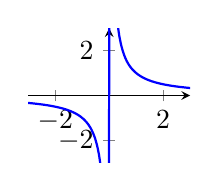
\begin{tikzpicture}
        \begin{axis}[ axis lines = center, xmin=-3, xmax=3, ymin=-3, ymax=3, scale = 0.3, samples=100]
            \addplot[blue, smooth, thick, unbounded coords = jump] {1/x};
        \end{axis}
    \end{tikzpicture}\\

    \noindent
    \textbf{Exponential Function}\\
    $y = 2^{x}$\\
    Key Points = \{(-2, 1/4), (-1, 1/2), (0,1), (1,2), (2,4)\}\\
    Domain = \{$\mathbb{R}$\} \\
    Range = \{ $y \epsilon \mathbb{R} | y > 0$\} \\

    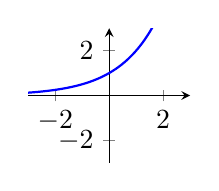
\begin{tikzpicture}
        \begin{axis}[ axis lines = center, xmin=-3, xmax=3, ymin=-3, ymax=3, scale = 0.3, samples=100]
            \addplot[blue, smooth, thick, unbounded coords = jump] {2^x};
        \end{axis}
    \end{tikzpicture}\\

    \end{multicols}

%----------------------------------------------------------

\newpage
\section{Domain and Range}

\textbf{Domain} - The set of all x values (input) \\
\textbf{Range} - The set of all y values (output) \\\\
\textbf{Symbols}
\begin{itemize}
    \item $\mathbb{R}$ - the set of real numbers
    \item $\mathbb{Z}$ - the set of integers
    \item $\epsilon$ - belongs to
    \item $\mid$ - such that
    \item $\eqslantless, <, \leqslant, >$
\end{itemize}

\noindent
\\For finite sets there are no duplicates and the values are in order.\\\\

\noindent
\textbf{Domain \& Range From Equations - Common Restrictions}\\
1. Cannot divide by zero\\
2. Cannot square root negatives\\
3. Vertex restrictions (use the graph)\\

%----------------------------------------------------------

\newpage
\section{The Inverse Function}

$f^{-1}(x)$
\begin{itemize}
    \item The inverse function is the "reverse" of the original function
    \item $f(x)$ operates in a specific way and order, $f^{-1}(x)$ will do the opposite operation in the reverse order
    \item Referred to as "inverse of f" or "f inverse"
\end{itemize} 

$(x,y) \epsilon f(x), (y,x) \epsilon f^{-1}(x)$\\

\noindent
Note:\\
$f(f^{-1}(x)) = f^{-1}(f(x))$ = x\\
$f(x)$ and $f^{-1}(x)$ "cancel" each other\\

\noindent
Steps to find the inverse:
\begin{enumerate}
    \item Given a list of points flip the coordinates\\
        (x,y) turns to (y,x)
    \item Given an equation in function notation\\
        - convert "y=" to "let f(x) = y"\\
        - switch x and y variables\\
        - solve for y\\
        - if the inverse expression is a function, convert back to $f^{-1}(x)$
    \item Given a discrete graph flip all points and replot
    \item Given a continuous graph choose select points to flip OR reflect graph in the line y = x
\end{enumerate} 

%----------------------------------------------------------

\newpage
\section{Transformations}

    \[ y = af(k(x-d))+c \]

    \noindent
    Where:\\
    - a and c affect the y-coordinate\\
    - k and d affect the x-coordinate

    \subsubsection*{Functions}

        \begin{multicols}{3}
        \noindent
        Quadratic Function\\
        $y = x^{2}$\\
        $y = a(k(x-d))^{2}+c$\\\\
        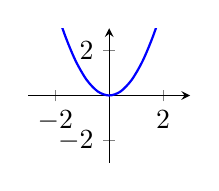
\begin{tikzpicture}
            \begin{axis}[scale = 0.3, axis lines = center, xmin=-3, xmax=3, ymin=-3, ymax=3]
                \addplot[blue,smooth, thick] {x^2};
            \end{axis}
        \end{tikzpicture}\\

        \noindent
        Root Function\\
        $y = \sqrt{x}$\\
        $y = a\sqrt{k(x-d)}+c$\\\\
        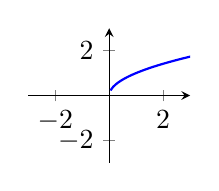
\begin{tikzpicture}
            \begin{axis}[ axis lines = center, xmin=-3, xmax=3, ymin=-3, ymax=3, scale = 0.3, samples=100]
                \addplot[blue, smooth, thick, unbounded coords = jump] {sqrt(x)};
            \end{axis}
        \end{tikzpicture}\\

        \columnbreak
        \noindent
        Cubic Function\\
        $y = x^{3}$\\
        $y = a(k(x-d))^{3}+c$\\\\
        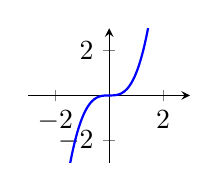
\begin{tikzpicture}
            \begin{axis}[ axis lines = center, xmin=-3, xmax=3, ymin=-3, ymax=3, scale = 0.3, samples=100]
                \addplot[blue, smooth, thick, unbounded coords = jump] {x^3};
            \end{axis}
        \end{tikzpicture}\\

        \noindent
        Absolute Value Func\\
        $y = |x|$\\
        $y = a|k(x-d)|+c$\\\\
        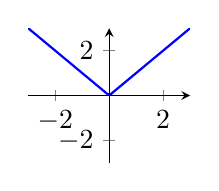
\begin{tikzpicture}
            \begin{axis}[ axis lines = center, xmin=-3, xmax=3, ymin=-3, ymax=3, scale = 0.3, samples=100]
                \addplot[blue, smooth, thick, unbounded coords = jump] {abs(x)};
            \end{axis}
        \end{tikzpicture}\\

        \columnbreak
        \noindent
        Reciprocal Function\\
        $y = \frac{1}{x}$\\
        $y = \frac{a}{k(x-d)}+c$\\\\
        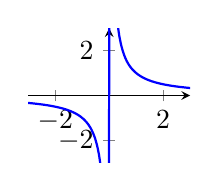
\begin{tikzpicture}
            \begin{axis}[ axis lines = center, xmin=-3, xmax=3, ymin=-3, ymax=3, scale = 0.3, samples=100]
                \addplot[blue, smooth, thick, unbounded coords = jump] {1/x};
            \end{axis}
        \end{tikzpicture}\\

        \noindent
        Exponential Func\\
        $y = 2^{x}$\\
        $y = a2^{k(x-d)}+c$\\\\
        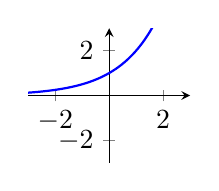
\begin{tikzpicture}
            \begin{axis}[ axis lines = center, xmin=-3, xmax=3, ymin=-3, ymax=3, scale = 0.3, samples=100]
                \addplot[blue, smooth, thick, unbounded coords = jump] {2^x};
            \end{axis}
        \end{tikzpicture}\\

        \end{multicols}

    %\newpage
    \noindent
    \textbf{Effects of Letters}

    \begin{multicols}{2}

    \noindent
    \textbf{a:} $ 0 < |a| < 1 $\\
    \noindent
    Vert. compression by a factor of $|a|$\\
    Multiply y values by $|a|$\\

    \noindent
    $|a| > 1$\\
    Vertical stretch by a factor of $|a|$\\
    Multiply y values by $|a|$\\

    \noindent
    $a < 0$\\
    Reflection over the x-axis\\
    Multiply y values by -1\\

    \columnbreak
    \noindent
    \textbf{k:} $ 0 < |k| < 1 $\\
    \noindent
    Horizontal stretch by a factor of $\frac{1}{|k|}$\\
    Multiply x values by $\frac{1}{|k|}$\\\\
    $|k| > 1$\\
    \noindent
    Horizontal compression by $\frac{1}{|k|}$\\
    Multiply x values by $\frac{1}{|k|}$\\\\
    $k<0$\\
    \noindent
    Reflection over the y-axis\\
    Multiply x values by -1

    \end{multicols}

    \begin{multicols}{2}
    \noindent \\\\
    \textbf{c:} $ c > 0 $ \\
    \noindent
    Shift up c units\\
    Add c to y values\\

    \noindent
    $c < 0$ \\
    Shift down c units\\
    Add c to y values\\

    \columnbreak
    \noindent  \\\\
    \textbf{d:} $d > 0$\\
    \noindent
    Shift right d units\\
    Add d to x values\\

    \noindent
    $d < 0$\\
    Shift left d units\\
    Add d to x values \\

    \end{multicols}

    \noindent
    \newpage
    Notes:\\
    - k must be factored out in order to determine the value of d\\
    - The order to complete transformations is:
    \begin{verbatim}
    1) Stretch/Compress
    2) Reflect
    3) Shift
    \end{verbatim}

%----------------------------------------------------------

\newpage
\section*{Piecewise Functions}

\textbf{Piecewise} - A \textbf{funciton} made up of two or more functions on given intervals.\\
\textbf{Notation Examle}\\
\[ \begin{cases} 
    function & restrictions \\
    x & 0 < x\leq 100 \\
    1 & 100 < x 
 \end{cases}
\]


%----------------------------------------------------------

\end{document}